\documentclass[12pt,a4paper]{article}

\usepackage[margin=1in]{geometry}

\usepackage{setspace}
\onehalfspacing

\usepackage{tikz}
\usetikzlibrary{positioning, arrows.meta}

\usepackage{float}

\usepackage{hyperref}

\begin{document}

\begin{titlepage}
\centering

\vspace*{1.5cm}

{\Large\textbf{ACTIVITIES AND FUNCTIONS OF}}\\[0.35cm] {\Large\textbf{STATISTICAL}}\\[0.35cm]
{\Large\textbf{DEPARTMENTS IN KERALA AND INDIA}}

\vspace{1.8cm}

{\large\textbf{A REPORT}}

\vspace{1.5cm}

{\Large\textit{Submitted By}}

\vspace{1.5cm}

{\large\textbf{ARYA T S (26150370)}}

\vspace{1.5cm}

{\large\textbf{MASTER OF TECHNOLOGY}}

\vspace{0.35cm}

{\large\textbf{ARTIFICIAL INTELLIGENCE AND SOFTWARE}}\\[0.35cm]{\Large\textbf{ENGINEERING}}

\vspace{1.5cm}

{\large\textbf{DEPARTMENT OF COMPUTER SCIENCE AND}}\\[0.35cm]{\large\textbf{ENGINEERING}}

\vspace{1.5cm}

{\large\textbf{COCHIN UNIVERSITY OF SCIENCE AND TECHNOLOGY}}

\vspace{0.35cm}

{\large\textbf{KOCHI, KERALA}}

\vspace{0.35cm}

{\large\textbf{SEPTEMBER 2026}}

\end{titlepage}

\section{Introduction}

Statistics is a field of study that involves collecting, organising, analysing, interpreting and presenting data. Governments use statistics to assess the social and economic conditions of a population and to understand the current situation of a region. Statistics produced or compiled through official statistical systems constitute official statistics. These statistics support planning, policy-making and decision-making at different levels of government. Statistical departments therefore play an important role in collecting, compiling, analysing and disseminating official statistics. This report examines the activities and functions of statistical departments in Kerala and India.

\section{Department of Economics and Statistics (DES)}

\subsection{Identity}

The Department of Economics and Statistics (DES) is the statistical agency of Kerala responsible for collecting, compiling, analysing, interpreting and disseminating statistical data relating to various sectors of the state. The Directorate of Economics and Statistics serves as the centre of the state statistical system and plays a key role in maintaining and providing official statistical information for Kerala.

\subsection{Role}

The Department of Economics and Statistics plays an important role in providing reliable statistical information for the planning and development of Kerala. It conducts statistical surveys and collects data relating to different sectors of the state economy and society. The collected data are compiled, analysed and disseminated to support government planning, policy formulation and decision-making. The department therefore serves as an important source of statistical information for understanding the social and economic conditions of the state.

\subsection{Organisation}

The Directorate of Economics and Statistics forms the central part of Kerala's statistical system and is headed by the Director, who is responsible for the technical and administrative functioning of the department. The Directorate is organized into divisions, which are further divided into sections dealing with specific subject areas.

\vspace{0.15cm}

At the district level, the department has District Statistical Offices, which are headed by Deputy Directors. At the taluk level, the Taluk Statistical Offices function as the lower-level statistical units of the department and are responsible for statistical activities at the local level.

\vspace{0.15cm}

In addition to the Directorate and its district and taluk offices, statistical cells function in various departments of the Kerala State Government. These cells are staffed by personnel from the Department of Economics and Statistics and collect, compile, analyse and disseminate statistical information relevant to the functions and requirements of their respective departments.

\begin{figure}[h]
\centering

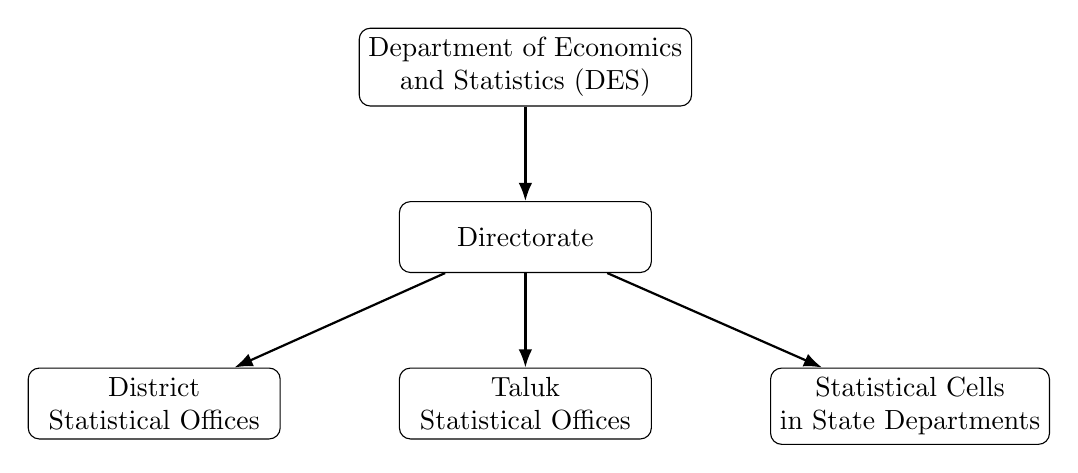
\begin{tikzpicture}[
    node distance=1.2cm and 1.5cm,
    box/.style={
        draw,
        rounded corners,
        align=center,
        minimum width=3.2cm,
        minimum height=0.9cm
    },
    arrow/.style={
        -{Latex},
        thick
    }
]

\node[box] (des) {Department of Economics\\and Statistics (DES)};

\node[box, below=of des] (directorate) {Directorate};

\node[box, below left=of directorate] (district)
    {District\\Statistical Offices};

\node[box, below=of directorate] (taluk)
    {Taluk\\Statistical Offices};

\node[box, below right=of directorate] (cells)
    {Statistical Cells\\in State Departments};

\draw[arrow] (des) -- (directorate);
\draw[arrow] (directorate) -- (district);
\draw[arrow] (directorate) -- (taluk);
\draw[arrow] (directorate) -- (cells);

\end{tikzpicture}

\caption{Organisational structure of the Department of Economics and Statistics}
\label{fig:des-organisation}

\end{figure}

\subsection{Functions and Activities}

The Department of Economics and Statistics carries out statistical activities covering a wide range of demographic, economic, agricultural, industrial and social sectors of Kerala. Its work includes the collection, compilation, analysis, interpretation and dissemination of statistical information required for understanding the conditions and development of the state.

In the area of population and demography, the department provides population statistics and vital statistics such as birth rate, death rate, infant mortality rate and maternal death ratio. In agriculture, it produces statistics on crop area, production, productivity, land utilisation and cost of cultivation. The department also prepares estimates of state and district income, including indicators such as Gross State Domestic Product and per-capita income.

DES also undertakes industrial and price-related statistical activities. These include the Annual Survey of Industries, the Index of Industrial Production and the collection and publication of consumer and market price statistics. In addition, the department produces socio-economic statistics relating to labour, housing, infrastructure, environment, gender and other sectors through surveys and other statistical programmes.

The collected data are further analysed and disseminated through datasets, statistical publications, reports, fact sheets, interactive dashboards and other data products. These activities enable statistical information to be made available for planning, policy formulation, research and decision-making in Kerala.

\begin{figure}[H]
\centering

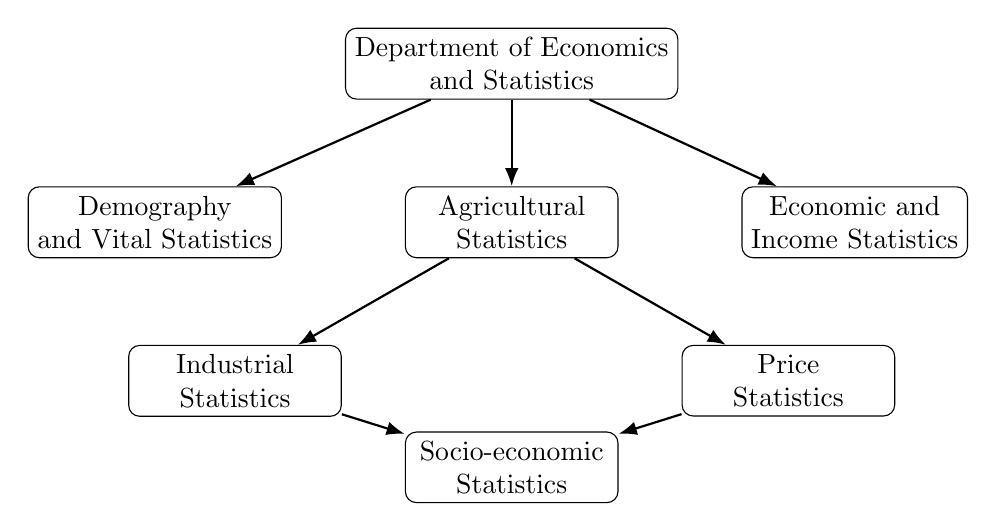
\begin{tikzpicture}[
    node distance=1.1cm and 0.8cm,
    box/.style={
        draw,
        rounded corners,
        align=center,
        minimum width=2.7cm,
        minimum height=0.85cm
    },
    arrow/.style={
        -{Latex},
        thick
    }
]

\node[box] (des) {Department of Economics\\and Statistics};

\node[box, below left=of des] (demo)
    {Demography\\and Vital Statistics};

\node[box, below=of des] (agri)
    {Agricultural\\Statistics};

\node[box, below right=of des] (economy)
    {Economic and\\Income Statistics};

\node[box, below left=of agri] (industry)
    {Industrial\\Statistics};

\node[box, below right=of agri] (prices)
    {Price\\Statistics};

\node[box, below=2.2cm of agri] (social)
    {Socio-economic\\Statistics};

\draw[arrow] (des) -- (demo);
\draw[arrow] (des) -- (agri);
\draw[arrow] (des) -- (economy);
\draw[arrow] (agri) -- (industry);
\draw[arrow] (agri) -- (prices);
\draw[arrow] (industry) -- (social);
\draw[arrow] (prices) -- (social);

\end{tikzpicture}

\caption{Major statistical activities of DES}
\label{fig:des-functions}

\end{figure}

\begin{figure}[H]
\centering

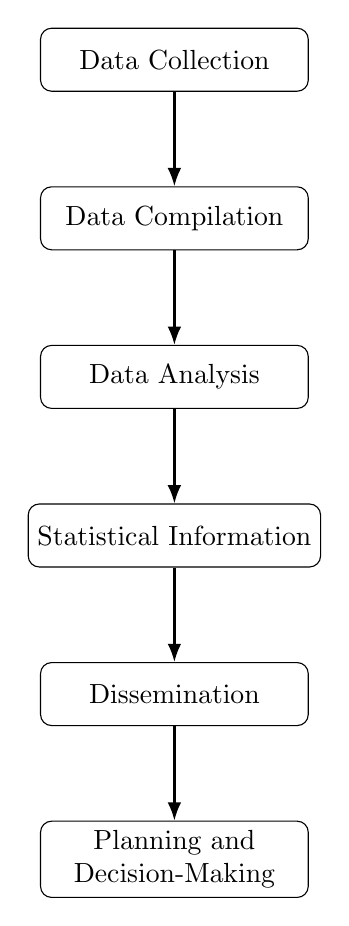
\begin{tikzpicture}[
    node distance=1.2cm,
    box/.style={
        draw,
        rounded corners,
        align=center,
        minimum width=3.4cm,
        minimum height=0.8cm
    },
    arrow/.style={
        -{Latex},
        thick
    }
]

\node[box] (collection) {Data Collection};
\node[box, below=of collection] (compilation) {Data Compilation};
\node[box, below=of compilation] (analysis) {Data Analysis};
\node[box, below=of analysis] (statistics) {Statistical Information};
\node[box, below=of statistics] (dissemination) {Dissemination};
\node[box, below=of dissemination] (decision) {Planning and\\Decision-Making};

\draw[arrow] (collection) -- (compilation);
\draw[arrow] (compilation) -- (analysis);
\draw[arrow] (analysis) -- (statistics);
\draw[arrow] (statistics) -- (dissemination);
\draw[arrow] (dissemination) -- (decision);

\end{tikzpicture}

\caption{Flow of statistical information and its use}
\label{fig:statistical-flow}

\end{figure}

\section{Statistical System of India}

\subsection{Identity}

The statistical system of India is responsible for producing, compiling, analysing and disseminating official statistics relating to various aspects of the country. At the central level, the Ministry of Statistics and Programme Implementation (MoSPI) is the principal ministry responsible for official statistics and statistical standards in India. The National Statistical Office (NSO), functioning under MoSPI, carries out major statistical activities including surveys, compilation of national accounts and other official statistical programmes.

\subsection{Role}

The statistical system of India provides statistical information required for understanding the country's demographic, social, economic and industrial conditions. The statistics produced through the system support government planning, policy formulation, monitoring of development programmes and research. It also establishes statistical standards and methodologies to promote consistency and comparability in official statistics.

\subsection{Organisation}

The Ministry of Statistics and Programme Implementation forms an important part of India's official statistical system. The National Statistical Office functions under MoSPI and carries out major statistical activities at the national level. The statistical system also involves other Central Ministries, Departments and State Governments, which collect and provide statistics relating to their respective areas of responsibility.

\subsection{Functions and Activities}

The statistical system of India covers a wide range of statistical activities. These include the compilation of national accounts and estimates of national income, population and demographic statistics, industrial statistics, price statistics, employment and socio-economic statistics and other sectoral statistics. The National Statistical Office conducts large-scale sample surveys to collect information on different aspects of the economy and society.

The statistical data obtained through surveys and administrative sources are processed, compiled, analysed and published through various statistical reports, datasets and other dissemination platforms. These activities provide reliable statistical information for planning, policy-making, economic analysis, research and decision-making at the national and state levels.

\begin{figure}[H]
\centering

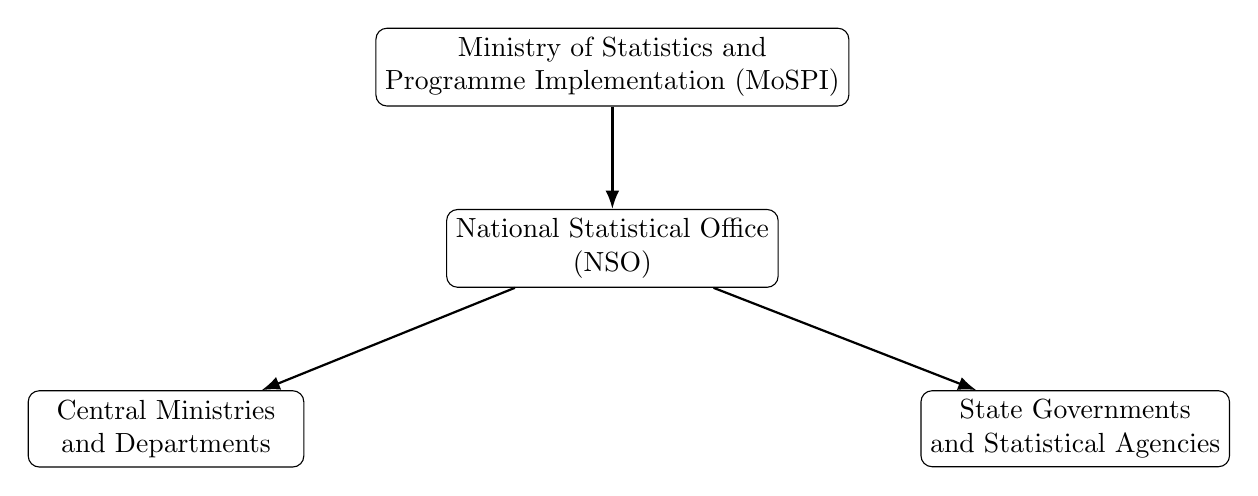
\begin{tikzpicture}[
    node distance=1.3cm and 1.8cm,
    box/.style={
        draw,
        rounded corners,
        align=center,
        minimum width=3.5cm,
        minimum height=0.9cm
    },
    arrow/.style={
        -{Latex},
        thick
    }
]

\node[box] (mospi)
    {Ministry of Statistics and\\Programme Implementation (MoSPI)};

\node[box, below=of mospi] (nso)
    {National Statistical Office\\(NSO)};

\node[box, below left=of nso] (central)
    {Central Ministries\\and Departments};

\node[box, below right=of nso] (states)
    {State Governments\\and Statistical Agencies};

\draw[arrow] (mospi) -- (nso);
\draw[arrow] (nso) -- (central);
\draw[arrow] (nso) -- (states);

\end{tikzpicture}

\caption{Major components of India's official statistical system}
\label{fig:india-statistical-system}

\end{figure}

\section{Conclusion}

Statistical departments play an important role in the production and dissemination of official statistics required for governance and development. In Kerala, the Department of Economics and Statistics carries out statistical activities covering demographic, agricultural, economic, industrial, price and socio-economic sectors. At the national level, the statistical system coordinated through the Ministry of Statistics and Programme Implementation and the National Statistical Office performs similar functions on a wider scale.

The activities of these statistical systems extend beyond the collection of data to its compilation, analysis, interpretation and dissemination. The resulting statistical information supports planning, policy formulation, research and decision-making. Thus, an organised statistical system is essential for understanding social and economic conditions and for supporting evidence-based development.

\newpage

\section*{References}

\begin{enumerate}

    \item Department of Economics and Statistics, Government of Kerala. 
    \textit{Department of Economics and Statistics}. 
    \url{https://ecostat.kerala.gov.in/}

    \item Department of Economics and Statistics, Government of Kerala. 
    \textit{Official Statistics and Statistical Activities of Kerala}. 
    \url{https://ecostat.kerala.gov.in/}

    \item Ministry of Statistics and Programme Implementation, Government of India. 
    \textit{Ministry of Statistics and Programme Implementation}. 
    \url{https://www.mospi.gov.in/}

    \item Ministry of Statistics and Programme Implementation, Government of India. 
    \textit{National Statistical Office}. 
    \url{https://www.mospi.gov.in/national-statistical-office}

\end{enumerate}

\end{document}
